% !TeX root = ../UrrutiaAnguiano_CandidaturaDefensa.tex
% !TeX spellcheck = es_MX 

\subsection{Teoría de película delgada}

{\setbeamertemplate{frametitle}[centertitle]{}
\begin{frame}{\underline{Campos, corrientes y cargas de exceso\footnotemark[1]}}
	{Contribución total del exceso}
	\vskip1em
\begin{columns}
	\column{\squeezethree}
	\begin{alertblock}{Sistema estratificado}
	\centering
		$$\vb{E}(\vb{r}) = \vb{E}^{>}(\vb{r}) \Theta(z) + \vb{E}^{<}(\vb{r}) \Theta(-z) + \vb{E}^\text{excess}(\vb{r})$$
		$$\vb{E}(\vb{r};\,z \to \pm \infty) \to  \vb{E}^{\gtrless}(\vb{r})$$
		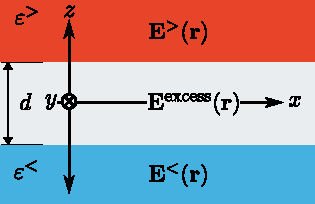
\includegraphics[scale = 1]{img/2-TFT/TFT-excess.pdf}
		
		\begin{itemize}
			\item  Tres medios semiinfinitos
			\item  $\varepsilon^\gtrless$ para medios en extremos
			\item $\vb{E}^{\gtrless}(\vb{r})$: Campo radiativo
			\item Descomposición válida para
				\begin{itemize}
					\item $\vb{B}(\vb{r})$ y $\vb{H}(\vb{r})$  
					\item $\vb{D}(\vb{r})$ 
					\item $\vb{J}_\text{ext}(\vb{r})$ y $\rho_\text{ext}(\vb{r})$  
				\end{itemize} 
		\end{itemize}
	\end{alertblock}
	
	\column{\squeezetwo}
	\begin{block}{Ecuaciones de Maxwell (Campos de exceso)}
		\begin{align*}
			\nabla\cdot\vb{D}^\text{excess}(\vb{r}) + \qty[D_\perp^>(\vb{r}_\parallel)-D_\perp^<(\vb{r}_\parallel)]\delta(z)  & = \rho^\text{excess}_\text{ext}(\vb{r})\\
			%	
			\nabla\cdot\vb{B}^\text{excess}(\vb{r}) + \qty[B_\perp^>(\vb{r}_\parallel)-B_\perp^<(\vb{r}_\parallel)]\delta(z)  & = 0\\
			%	
			\nabla\times\vb{E}^\text{excess}(\vb{r}) + \vu{e}_\perp \times \qty[\vb{E}^>_\parallel(\vb{r}_\parallel)-\vb{E}^<_\parallel(\vb{r}_\parallel)]\delta(z) & = +i\omega\vb{B}^\text{excess}(\vb{r})\\
			%	
			\nabla\times\vb{H}^\text{excess}(\vb{r}) + \vu{e}_\perp \times \qty[\vb{H}^>_\parallel(\vb{r}_\parallel)-\vb{H}^<_\parallel(\vb{r}_\parallel)]\delta(z) & = \vb{J}^\text{excess}_\text{ext}(\vb{r}) -i\omega\vb{D}^\text{excess}(\vb{r})
		\end{align*}
	\end{block}

	\begin{block}{\centering Límite de película delgada}
	\centering
		$$\vb{E}(\vb{r}) = \vb{E}^{>}(\vb{r}) \Theta(z) + \vb{E}^{<}(\vb{r}) \Theta(-z) + \vb{E}^\text{film}(\vb{r}_\parallel) \delta(z)$$
		$$	\vb{E}^\text{film}(\vb{r}_\parallel)
		= \int_{-\infty}^{\infty} \vb{E}^\text{excess}(\vb{r}) \dd{z}
		= \qty(\int_{-\infty}^{\infty} \vb{E}^\text{excess}(\vb{r})\exp(i k_z z) \dd{z})\eval_{k_z = 0}$$
	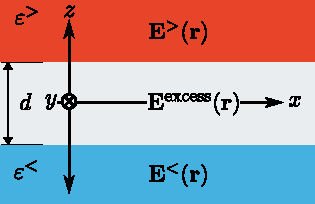
\includegraphics[scale = 1]{img/2-TFT/TFT-excess.pdf}
		\quad
	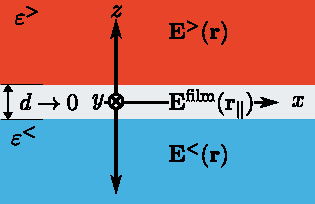
\includegraphics[scale = 1]{img/2-TFT/TFT-film.pdf}
\end{block}		
\end{columns}
\begin{textblock*}{80mm}(145mm,137.5mm)
	\begin{flushleft}
		\scriptsize
		\rule{30mm}{.5pt}\\
		\footnotemark[1]\fullcite{bedeaux_optical_2004}
	\end{flushleft}
\end{textblock*}

\end{frame}
}


\begin{frame}[c]{\underline{Teoría de película delgada (TFT)}}
	{Condiciones de frontera modificadas\footnotemark[1]}
\centering
\begin{tikzpicture}[node distance=10 mm and 15mm]
	\path (0,0) node [concept]  (meta) {\large Ecuaciones de Maxwell para campos de exceso};

	\node[concept, below right =of meta,yshift=-15mm ] (PM) {Ecuaciones constitutivas};
	\node[below =of PM, yshift=15mm] (const-eq) {\begin{minipage}{50mm}
			\begin{align*}
				\vb{P}^\text{film}(\vb{r}_\parallel) &= 
				\gamma\,\big\langle\vb{E}^\text{film}_\parallel(\vb{r}_\parallel)\big\rangle +
				\beta \,\big\langle {D}^\text{film}_\perp(\vb{r}_\parallel)\big\rangle \vu{e}_\perp\\
				\vb{M}^\text{film}(\vb{r}_\parallel) &= \vb{0}
			\end{align*}
	\end{minipage}};	
	
	\node [flowbox, fb-highlight, below right =of const-eq, xshift=-5mm] (cf) {\fbtitle{Condiciones de frontera}
		\nodepart{two}
		\begin{minipage}{50mm}
			\begin{align*}
	\qty[D_\perp^>(\vb{r}_\parallel)-D_\perp^<(\vb{r}_\parallel)]  & = -\nabla_\parallel\cdot\vb{P}_\parallel^\text{film}(\vb{r}_\parallel)\\
	%	
	\qty[B_\perp^>(\vb{r}_\parallel)-B_\perp^<(\vb{r}_\parallel)]  & = -\nabla_\parallel\cdot\vb{M}_\parallel^\text{film}(\vb{r}_\parallel)\\
	%	
	\qty[\vb{E}^>_\parallel(\vb{r}_\parallel)-\vb{E}^<_\parallel(\vb{r}_\parallel)] & = -i{\omega}\vu{e}_\perp\times \vb{M}^\text{film}_\parallel(\vb{r}_\parallel)-\nabla_\parallel P_\perp^\text{film}(\vb{r}_\parallel)\\
	%	
	\qty[\vb{H}^>_\parallel(\vb{r}_\parallel)-\vb{H}^<_\parallel(\vb{r}_\parallel)] & = +i{\omega}\vu{e}_\perp\times \vb{P}^\text{film}_\parallel(\vb{r}_\parallel)-\nabla_\parallel M_\perp^\text{film}(\vb{r}_\parallel)
			\end{align*}
	\end{minipage}};

	
	\draw[hidden] (meta.south) |-
	node[above,text=sdgrayFC,font=\small,anchor=east]
		{\begin{minipage}{30mm}
			\begin{flushright}
			Límite de película delgada\\
			Transformada de Fourier en $z$\\
			$k_z = 0$
		\end{flushright}
		\end{minipage}}
	node[below, near end,text=sdgrayFC,font=\small,anchor=south]
	{$\big\langle a^\text{film} (\vb{r}_\parallel)\big\rangle~=~\dfrac12[a^>(\vb{r}_\parallel) + a^<(\vb{r}_\parallel)]$}
	(PM.west);

	\draw[hidden] (PM.east) -| (cf.north);
	
	
	\node[below =of meta, yshift=-50mm] (diagrama) {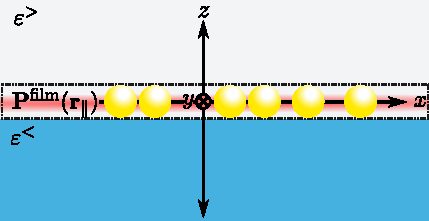
\includegraphics[scale=1]{img/2-TFT/monolayer.pdf}};
	\node[right=of diagrama, xshift=-18mm] {\begin{minipage}{60mm}
			\begin{itemize}
				\item $\gamma = \dfrac23 \dfrac{\Theta}{V_\text{sp}} \qty( \dfrac{\alpha_\text{sp}}{1 + A \alpha_\text{sp}})$
				\item $\beta =\dfrac23 \dfrac{\Theta}{\varepsilon_i^2 V_\text{sp}} \qty(\dfrac{\alpha_\text{sp}}{1 + 2 A \alpha_\text{sp}})$
				\item $\alpha_\text{sp} = 3  \varepsilon_t V_\text{sp} \qty(\dfrac{\varepsilon_\text{sp} - \varepsilon_t}{\varepsilon_\text{sp} + 2 \varepsilon_t})$
				\item $A = \dfrac{\varepsilon_i - \varepsilon_t}{\varepsilon_i + \varepsilon_t}$
			\end{itemize}
	\end{minipage}};
\end{tikzpicture}

\begin{textblock*}{80mm}(145mm,137.5mm)
	\begin{flushleft}
		\scriptsize
		\rule{30mm}{.5pt}\\
		\footnotemark[1]\fullcite{bedeaux_optical_2004}
	\end{flushleft}
\end{textblock*}
\end{frame}


\begin{frame}{\underline{Teoría de película delgada (TFT)}}
	{Coeficientes de Fresnel modificado\footnotemark[1]}
\begin{columns}
	\column{\squeezethree}
		\centering
		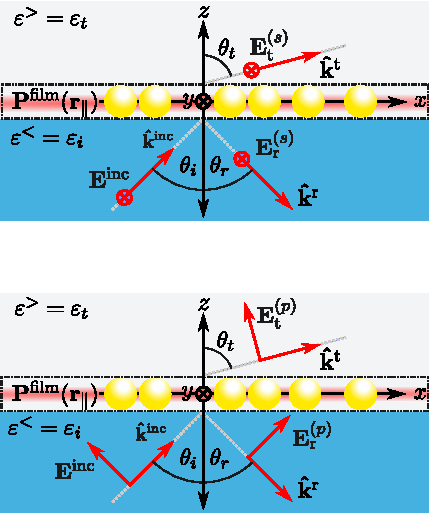
\includegraphics[scale = 1]{img/2-TFT/Fresnel.pdf}
	\column{\squeezetwo}
		\begin{block}{Polarización: $s$}
		\begin{align*}
			r^{(s)}_\text{TFT}(\theta_i) =&  \frac{ n_i \cos\theta_i - n_t\cos\theta_t + i (\omega/c)\gamma }
			{ n_i \cos\theta_i + n_t\cos\theta_t - i (\omega/c)\gamma } \\
			t^{(s)}_\text{TFT}(\theta_i) =& \frac{ 2 n_i \cos\theta_i}
			{ n_i \cos\theta_i + n_t\cos\theta_t - i (\omega/c)\gamma },
		\end{align*}
		\end{block}
		
		\vskip3em
		\begin{block}{Polarización: $p$}
		\begin{align*}
				r^{(p)}_\text{TFT}(\theta_i) &= \frac{ \kappa_-(\omega) - i (\omega/c) \gamma\cos\theta_i\cos\theta_t +
															i (\omega/c)  n_i n_t \varepsilon_i \beta \sin^2 \theta_i }
													{ \kappa_+(\omega) - i (\omega/c) \gamma\cos\theta_i\cos\theta_t -
															i (\omega/c)  n_i n_t \varepsilon_i \beta \sin^2 \theta_i }\\
			t^{(p)}_\text{TFT}(\theta_i) &=  \frac{ n_i \cos\theta_i \qty(1-\qty(\omega/2c)^2\varepsilon_{i}\gamma\beta \sin^{2}\theta_i) }
													{ \kappa_+(\omega) - i (\omega/c) \gamma\cos\theta_i\cos\theta_t -
													i (\omega/c)  n_i n_t \varepsilon_i \beta \sin^2 \theta_i }\\ \\
			\kappa_{\pm}(\omega) &= \bigg( n_t \cos\theta_i \pm n_i \cos\theta_t \bigg)
									\qty[1-\qty(\frac{\omega}{2c})^2\varepsilon_{i}\gamma\beta \sin^{2}\theta_i]
		\end{align*}
		\end{block}
\end{columns}
\begin{textblock*}{80mm}(145mm,137.5mm)
	\begin{flushleft}
		\scriptsize
		\rule{30mm}{.5pt}\\
		\footnotemark[1]\fullcite{bedeaux_optical_2004}
	\end{flushleft}
\end{textblock*}

\end{frame}